\documentclass[a4paper, 12pt]{article}
\usepackage[margin=2.5cm]{geometry}

% \usepackage{cmap}
% \usepackage[T1,T2A]{fontenc}
% \usepackage[utf8]{inputenc}
% \usepackage[english,ukrainian]{babel}
\usepackage{amsmath, amssymb, amsfonts}
\usepackage{fancyhdr}
\usepackage{mdframed}
\usepackage{graphicx}
\usepackage{pgfplots}

% set up headers
\pagestyle{fancy}
\setlength{\headheight}{15pt}
\fancyhead[R]{Oleh Shkalikov}
\fancyhead[L]{CMS-COR-SAP}
\fancyhead[C]{{Exercise 1}}

% disable wrapping
\tolerance=1
\emergencystretch=\maxdimen
\hyphenpenalty=10000
\hbadness=10000

% usable commands and definitions
\DeclareMathOperator{\R}{\mathbb{R}}
\DeclareMathOperator{\N}{\mathbb{N}}
\DeclareMathOperator{\E}{\mathbb{E}}
\DeclareMathOperator{\var}{var}

\newcommand{\rbra}[1]{\left( #1 \right)}
\newcommand{\sbra}[1]{\left[ #1 \right]}
\newcommand{\fract}[2]{\dfrac{\mathstrut #1}{\mathstrut #2}}

\newcommand{\task}[2]{
    \item #1
    \begin{mdframed} \textbf{Solution. } #2 \end{mdframed}
}

\title{CMS-COR-SAP. Exercise 1}
\author{Oleh Shkalikov}

\begin{document}

\maketitle

\begin{enumerate}
    \item Twins can be monozygotic (M) or dizygotic (D). Monozygotic
          twins are always of the same sex, but dizygotic twins can be
          of opposite sex. Assuming that two sexes are equally probable:
          \begin{enumerate}
              \task{What are the probabilities of each of the combinations
                  of sexes for monozygotic and dizygotic twins?}
              {Let $A$ be male and $B$ -- a female. In the case of monozygotic
                  twins it is impossible to have different sex children, thus probabilities
                  of different sex is equal to $0$ and, due to the balance between
                  sexes, probabilities of same sex twins for both sex is equal to $\frac{1}{2}$
                  \begin{align*}
                      P(AA | M) = P(BB | M) = \frac{1}{2} \\
                      P(AB | M) = P(BA | M) = 0
                  \end{align*}

                  In the case of dizygotic twins, due to the equality
                  between sexes and independence of child every combinations is equally
                  probable and equals to $\frac{1}{4}$
                  \begin{align*}
                      P(AA | D) = P(BB | D) = P(AB | D) = P(BA | D) = \frac{1}{4} = \frac{1}{2} \cdot \frac{1}{2}
                  \end{align*}
              }
              \task{What is the probability of having twins, monozygotic OR dizygotic,
                  that are both girls?}{Let's use formula of total probability:
                  \[
                      P(BB) = P(BB | M) P(M) + P(BB | D) P(D) = \frac{1}{2}P(M) + \frac{1}{4}P(D)
                  \]
                  Unfortunately, probabilities of dizygotic and monozygotic twins
                  haven't been provided so suppose they are equal, then:
                  \[
                      P(BB) = \frac{1}{2} \cdot \frac{1}{2} + \frac{1}{4} \cdot \frac{1}{2} = \frac{3}{8}
                  \]
              }
              \task{Knowing that the twins are both boys, what is the probability that they are monozygotic?}
              {For solve this task we are supposed to use Bayes theorem
                  \[
                      P(M | AA) = \frac{P(AA | M) P(M)}{P(AA)}
                  \]
                  Probability of having both boys is calculated as well as probability
                  of having two girls, with use of rule of total probability
                  \[
                      P(AA) = P(AA | M) P(M) + P(AA | D) P(D) = \frac{1}{2}P(M) + \frac{1}{4}P(D)
                  \]
                  So, making the same assumption about probability of dizygotic and monozygotic twins
                  as in the previous subtask, we have
                  \[
                      P(M | AA) = \frac{\frac{1}{2} P(M)}{\frac{1}{2}P(M) + \frac{1}{4}P(D)} =
                      \frac{\frac{1}{4}}{\frac{3}{8}} = \frac{2}{3}
                  \]
              }
          \end{enumerate}
          \task{Suppose a red ($r$) and blue ($b$) dice are tossed and their sum is $s = r + b$. What is the
              probability mass function of $x$? Make a table and plot out the PMF.}
          {
              We suppose that dices are balanced so every result is equally probable as some other one. It is obvious,
              that it is impossible to get more than $12$ and less than $2$ as the sum $s$. So
              we have to calculate PMF for $s = \overline{2, 12}$, for all other number probability is equal to $0$.
              To calculate this probability we have to count all combinations of dices
              which has sum $s$ and divide this number by total number of combinations $6 \cdot 6 = 36$.
              Thus, we have the following result:

              \begin{center}
                  \begin{tabular}{|c|c|c|c|c|c|c|c|c|c|c|c|}
                      \hline
                      $s$ & $2$             & $3$             & $4$             & $5$             & $6$             & $7$             & $8$             & $9$             & $10$            & $11$            & $12$            \\
                      \hline
                      PMF & $\fract{1}{36}$ & $\fract{2}{36}$ & $\fract{3}{36}$ & $\fract{4}{36}$ & $\fract{5}{36}$ & $\fract{6}{36}$ & $\fract{5}{36}$ & $\fract{4}{36}$ & $\fract{3}{36}$ & $\fract{2}{36}$ & $\fract{1}{36}$ \\
                      \hline
                  \end{tabular}
              \end{center}

              And having this table we can plot a graph of PMF.
              \begin{center}
                  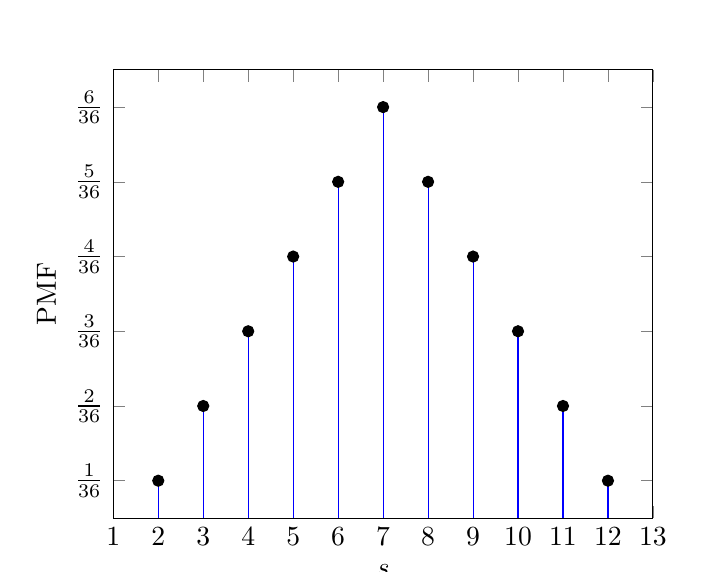
\begin{tikzpicture}
                      \begin{axis}[xlabel={$s$},
                              ylabel={PMF},
                              xtick distance={1},
                              ytick distance={1},
                              yticklabels={0, 0, $\frac{1}{36}$, $\frac{2}{36}$, $\frac{3}{36}$,
                                      $\frac{4}{36}$, $\frac{5}{36}$, $\frac{6}{36}$}
                          ]
                          \addplot[ycomb, color=blue, mark options={black}, mark=*] coordinates {(2,1)(3,2)(4,3)(5,4)(6,5)
                                  (7,6)(8,5)(9,4)(10, 3)(11, 2)(12, 1)};
                      \end{axis}
                  \end{tikzpicture}
              \end{center}
          }
    \item Suppose two balanced dice ($X$ and $Y$) are thrown. Make a table to solve the following:
          \begin{enumerate}
              \task{What is the joint probability of X and Y if Y is greater than X?}
              {
                  It is not possible to have $X=6$, because $X$ has to be less than $Y$ and maximum value of $Y$ is $6$.
                  So, first of all we will get $X$ from $5$ possible equally probable option with probability $\frac{1}{5}$.
                  The similar situation with $Y$: if $Y$ is greater than $X$ than it can't be equal
                  to $1$. But having $X$ we know, that $Y$ should be greater, so
                  it limits possible values for $Y$, for example: if $X=3$, then our possible choice is from a set
                  $\{4, 5, 6\}$. And of course this option is uniformly distributed (for this example
                  every option have probability $\frac{1}{3}$). Thus, apply the same logic for the rest cases,
                  we can calculate every conditional probability $P(X \cap Y | Y > X)$.
                  \begin{center}
                      \begin{tabular}{|c|c|c|c|c|c|c|}
                          \hline
                          $X / Y$ & $1$ & $2$                               & $3$                               & $4$                               & $5$                               & $6$                               \\
                          \hline
                          $1$     & 0   & $\fract{1}{5} \cdot \fract{1}{5}$ & $\fract{1}{5} \cdot \fract{1}{5}$ & $\fract{1}{5} \cdot \fract{1}{5}$ & $\fract{1}{5} \cdot \fract{1}{5}$ & $\fract{1}{5} \cdot \fract{1}{5}$ \\
                          \hline
                          $2$     & 0   & 0                                 & $\fract{1}{5} \cdot \fract{1}{4}$ & $\fract{1}{5} \cdot \fract{1}{4}$ & $\fract{1}{5} \cdot \fract{1}{4}$ & $\fract{1}{5} \cdot \fract{1}{4}$ \\
                          \hline
                          $3$     & 0   & 0                                 & 0                                 & $\fract{1}{5} \cdot \fract{1}{3}$ & $\fract{1}{5} \cdot \fract{1}{3}$ & $\fract{1}{5} \cdot \fract{1}{3}$ \\
                          \hline
                          $4$     & 0   & 0                                 & 0                                 & 0                                 & $\fract{1}{5} \cdot \fract{1}{2}$ & $\fract{1}{5} \cdot \fract{1}{2}$ \\
                          \hline
                          $5$     & 0   & 0                                 & 0                                 & 0                                 & 0                                 & $\fract{1}{5}$                    \\
                          \hline
                          $6$     & 0   & 0                                 & 0                                 & 0                                 & 0                                 & 0                                 \\
                          \hline
                      \end{tabular}
                  \end{center}
              }
              \task{What is the marginal distribution of Y (prob. of values of Y for all X)?}
              {I suppose, that this subtask don't refer to previous one, so in this case distribution of $Y$ is
                  uniform and every possible result $\overline{1, 6}$ has probability $\frac{1}{6}$.}
              \task{What is the conditional probability that X = 2 given Y = 1?}
              {
                  Let's expand our conditional probability by definition:
                  \[
                      P(X=2 | Y=1) = \frac{P(X=2 \cap Y=1)}{P(Y=1)}
                  \]
                  But $X$ and $Y$ are independent, so we have:
                  \[
                      P(X=2 | Y=1) = P(X=2) = \frac{1}{6}
                  \]
              }
          \end{enumerate}
    \item Expectation of a sum and of a product
          \begin{enumerate}
              \task{What is the expectation of $ax + by+c$, where $a$, $b$, and $c$ are constants and $x$ and $y$ are
                  random variables?}
              {Expectation of random variable $\xi$ with CDF $F(x)$ is an
                  Lebesgue-Stieltjes integral:
                  \[
                      \E \xi = \int\limits_{-\infty}^{\infty} \xi dF(\xi)
                  \]
                  So, expectation of an constant value $c$ is (we apply the property of CDF and integral):
                  \[
                      \E c = \int\limits_{-\infty}^{\infty} c dF(c) = c \int\limits_{-\infty}^{\infty} dF(c) = c \cdot 1 = c
                  \]
                  Next, applying linearity of integral we have:
                  \[
                      \E \rbra{ax + by + c} = a \E x + b \E y + c
                  \]
              }
              \task{What is the expectation of $xy$ if $x$ and $y$ are independent?}
              {
                  By definition expectation of $xy$ is ($F$ is a CDF):
                  \[
                      \E xy = \int\limits_{-\infty}^{\infty} s \cdot t \cdot dF_{xy}(s, t)
                  \]
                  But, due to the independence of $x$ and $y$, we have that
                  $F_{xy} = F_x \cdot F_y$, then:
                  \begin{multline*}
                      \E xy = \int\limits_{-\infty}^{\infty} s \cdot t \cdot dF_x(s) dF_y(t) = \\
                      \rbra{\int\limits_{-\infty}^{\infty} s dF_x(s)}
                      \rbra{\int\limits_{-\infty}^{\infty} s dF_y(s)} = \E x \cdot \E y
                  \end{multline*}
              }
          \end{enumerate}
    \item Suppose you have an alarm clock that rings after a random time $t$ that is exponentially
          distributed with rate $\lambda$ ($t \sim Exp(\lambda)$).
          \begin{enumerate}
              \task{What is the probability that the alarm clock rings for the 1st time after the lst hour?
              }
              {
              Let's calculate a probability using PDF (1 hour is equal to 3600 seconds):
              \[
                  P(t > 3600) = \int\limits_{3600}^{\infty} \lambda e^{-\lambda x} dx =
                  -e^{-\lambda x} \big|_{3600}^{\infty} = e^{-3600 \lambda}.
              \]
              }
              \task{What is the probability that the alarm clock rings for the Ist time after the 2nd hour?}
              {
              Let's calculate a probability using PDF (2 hour is equal to 7200 seconds):
              \[
                  P(t > 3600) = \int\limits_{7200}^{\infty} \lambda e^{-\lambda x} dx =
                  -e^{-\lambda x} \big|_{7200}^{\infty} = e^{-7200 \lambda}.
              \]
              }
              \task{If you knew that the alarm clock will not ring within the 1st hour, what is the probability
                  that it will ring for the lst time after the 2nd hour?}
              {
                  We calculate it using a definition of conditional probability:
                  \[
                      P(t > 7200 | t > 3600) = \frac{P(t > 7200 \cap t > 3600)}{P(t > 3600)}
                  \]
                  But, let's see that $\{t > 7200 \}$ is only a subset of event $\{ t > 3600 \}$ so,
                  joint probability is equal to probability of a subset, so:
                  \[
                      P(t > 7200 | t > 3600) = \frac{P(t > 7200)}{P(t > 3600)} = \frac{e^{-7200 \lambda}}{e^{-3600 \lambda}} = e^{-3600 \lambda} = P(t > 3600)
                  \]
              }
          \end{enumerate}
    \item A popcorn maker pops corn according to a Poisson process with a rate of $1$ corn kernel per
          second.
          \begin{enumerate}
              \task{What is the probability mass function of the number of kernels popped in 10 seconds?}
              {
                  By definition Poisson process is a stochastic process $(N(t),~t~\geq~0)$ which
                  satisfy the following properties:
                  \begin{itemize}
                      \item $N(0) = 0$
                      \item has independent increments: for any $0 \leq t_1 < \dots < t_m$, the increments
                            $N(t_1), N(t_2) - N(t_1), \dots N(t_m) - N(t_{m-1}) $ are independent
                      \item has homogenous increments: for any $t > s \geq 0$ the increment is
                            distributed such $N(t) - N(s) \stackrel{d}{=} N(t-s)$
                      \item $P(N(t) \geq 2) = o(t),\ t\rightarrow 0+$
                      \item $P(N(t) = 1) \sim \lambda t,\ t\rightarrow 0+$
                  \end{itemize}

                  Let's try to derive PMF for every possible $t \geq 0$. Let $p_k = P(N(t) = k)$, then
                  using homogeneity and independence of increments we have:
                  \begin{multline*}
                      p_0(t + \delta t) - p_0(t) = P(N(t+ \delta t) = 0) - P(N(t) = 0) \stackrel{hom}{=} \\
                      P(N(t) = 0, N(t + \delta t) - N(t) = 0) - P(N(t) = 0) \stackrel{ind}{=} \\
                      P(N(t) = 0) P(N(t + \delta t) - N(t) = 0) - P(N(t) = 0) \stackrel{hom}{=} \\
                      P(N(t) = 0) \rbra{P(N(\delta t) = 0) - 1} = -p_0(t) P(N(\delta t) \neq 0)
                  \end{multline*}

                  Let's divide this equality by $\delta t$ and expand last probability:
                  \[
                      \frac{p_0(t + \delta t) - p_0(t)}{\delta t} = -p_0(t)
                      \rbra{\frac{P(N(\delta t) = 1)}{\delta t} +
                          \frac{P(N(\delta t) \geq 2)}{\delta t} }
                  \]
                  Using the two last properties of Poisson process and suppose $\delta t \rightarrow 0$ we
                  get a differential equation:
                  \[
                      \begin{cases}
                          p_0'(t) = - \lambda p_0(t) \\
                          p_0(0) = 1
                      \end{cases} \implies
                      p_0(t) = e^{-\lambda t}
                  \]

                  Let's discover $p_k(t), k > 0$:
                  \begin{multline*}
                      p_k(t + \delta t) - p_k(t) = P(N(t + \delta t) = k) - P(N(t) = k) \stackrel{hom}{=} \\
                      \sum\limits_{j=0}^{k} P(N(t) = j, N(t + \delta t) - N(t) = k - j) - P(N(t) = k) \stackrel{ind}{=} \\
                      \sum\limits_{j=0}^{k} P(N(t) = j) P(N(\delta t) = k - j) - P(N(t) = k) \stackrel{4\ prop.}{=} \\
                      p_k(t) P(N(\delta t) = 0) + p_{k-1}(t) \cdot P(N(\delta t) = 1) + o(\delta t) - p_k(t) = \\
                      -p_k(t) P(N(\delta t) \geq 1  ) + p_{k-1}(t) \cdot P(N(\delta t) = 1) + o(\delta t)
                  \end{multline*}
                  Divide this equality by $\delta t$ and suppose $\delta t \rightarrow 0$ then:
                  \[
                      \begin{cases}
                          p_0'(t) = - \lambda p_k(t) + \lambda p_{k-1}(t) \\
                          p_k(0) = 0
                      \end{cases} \implies
                      p_0(t) = e^{-\lambda t}
                  \]
                  Let's notice that
                  \[
                      \rbra{e^{\lambda t} p_k(t)}' = e^{\lambda t} \rbra{\lambda p_k(t) + p'_k(t)} =
                      \lambda e^{\lambda t} p_{k-1}(t)
                  \]
                  Therefore:
                  \[
                      p_k(t) = \lambda e^{-\lambda t} \int\limits_0^t e^{\lambda s} p_{k-1}(s) ds
                  \]
                  Then:
                  \[
                      p_1(t) = \lambda e^{-\lambda t} \int\limits_0^t e^{\lambda s} e^{-\lambda s} ds = \lambda t e^{-\lambda t}
                  \]
                  Let it be a base of an induction. So, the next stage is a induction step: let
                  $p_{k-1}(t) = e^{-\lambda t} \frac{(\lambda t)^{k-1}}{(k-1)!}$. Is is obvious that $p_1$ satisfy this
                  assumption. So,
                  \begin{multline*}
                      p_k(t) = \lambda e^{-\lambda t} \int\limits_0^t e^{\lambda s} e^{-\lambda s} \frac{(\lambda s)^{k-1}}{(k-1)!} ds = \\
                      \lambda^k e^{-\lambda t} \int\limits_0^t \frac{(s)^{k-1}}{(k-1)!} ds =
                      e^{-\lambda t} \frac{(\lambda t) ^ k}{k!}
                  \end{multline*}

                  Thus, $N(t) \sim Poiss(\lambda t)$ and therefore
                  $p_k(10) = e^{-10} \frac{(10)^k}{k!}, k \in \N_0$
              }
              \task{What is the mean and variance of of the number of kernels popped in 10 seconds?}
              {
                  The mean and variance simply equal to mean and variance of
                  Poisson random variable with parameter $10 \cdot 1 = 10$, so
                  $\E N(10) = 10$, $\var N(10) = 10$.
              }
          \end{enumerate}
\end{enumerate}
\end{document}